\chapter{Conjugate gradient.}
\graphicspath{{chapters/05_conjugate_gradient/figures}}
\begin{abstract}
This chapter develops the method of conjugate directions, the linear
conjugate-gradient algorithm, its convergence behavior on SPD systems,
preconditioning, and the basic nonlinear conjugate-gradient family.
\end{abstract}
\tikzset{
  ch5-figbox/.style={rounded corners=3pt, draw=slate!28, fill=lightgray!20, line width=0.4pt},
  ch5-line/.style={draw=slate!76, line width=0.55pt, line cap=round},
  ch5-accent/.style={draw=teal!75!black, fill=teal!10, line width=0.55pt},
  ch5-warm/.style={draw=crimson!78!black, fill=crimson!8, line width=0.55pt},
  ch5-arrow/.style={-latex, draw=slate!82, line width=0.75pt, line cap=round, shorten >=1pt, shorten <=1pt},
  ch5-label/.style={font=\footnotesize, text=slate!95},
  ch5-small/.style={font=\scriptsize, text=slate!92},
  ch5-node/.style={font=\footnotesize, inner sep=1.6pt, rounded corners=1pt, fill=white, text=slate!95},
}

It is useful to place conjugate gradients between the two methods we already
know best. If the cost of one objective/gradient evaluation is $O(q)$, then a
rough comparison is
\begin{table}[ht]
  \centering
  \begin{tabular}{@{}lcc@{}}
    \toprule
    Method & Memory & Per-iteration compute\\
    \midrule
    Gradient descent (GD) & $O(n)$ & $O(q + n)$\\
    Newton (dense) & $O(n^2)$ & $O(qn+n^3)$\\
    \bottomrule
  \end{tabular}
  \caption{Rough per-iteration memory and computational cost for the two
  benchmark methods from earlier chapters. Here $n$ is the dimension and $q$
  is the cost of one objective/gradient evaluation. The Newton row assumes a
  dense Hessian and a direct solve via a matrix factorization.}
  \label{tab:ch5-gd-newton-cost}
\end{table}
so gradient descent is cheap but may zig-zag, while Newton is geometrically
better but much more expensive. Conjugate gradients are designed to keep the
storage and per-step structure much closer to gradient descent while still
using the quadratic geometry induced by Newton method.

\section{The method of conjugate directions}
\label{sec:ch5-conjugate-directions}
We begin with the quadratic problem
\begin{equation}
  \label{eq:ch5-quadratic}
  f(\mathbf{x})=\frac12 \mathbf{x}^{\top}\mathbf{A}\mathbf{x}
  -\mathbf{b}^{\top}\mathbf{x}
  \to \min_{\mathbf{x}\in\mathbb{R}^n},
  \qquad
  \mathbf{A}=\mathbf{A}^{\top}\succ 0.
\end{equation}
Its gradient is
\[
  \nabla f(\mathbf{x})=\mathbf{A}\mathbf{x}-\mathbf{b},
\]
so the optimality condition is the linear system
\[
  \mathbf{A}\mathbf{x}=\mathbf{b}.
\]
This is the best starting point to see why CG works. Afterwards, we
will consider more complex cases.

\subsection{Exact line search on a quadratic}
Suppose we move from $\mathbf{x}_k$ along a direction $\mathbf{d}_k$:
\[
  \mathbf{x}_{k+1}=\mathbf{x}_k+\alpha_k\mathbf{d}_k.
\]
For the quadratic \eqref{eq:ch5-quadratic}, exact line search is explicit
and we don't need Armijo--Wolfe. Let
\[
  \varphi_k(\alpha):=f(\mathbf{x}_k+\alpha \mathbf{d}_k),
  \qquad
  \mathbf{g}_k:=\nabla f(\mathbf{x}_k)=\mathbf{A}\mathbf{x}_k-\mathbf{b}.
\]
Then
\[
  \varphi_k'(\alpha)
  =(\mathbf{g}_k+\alpha \mathbf{A}\mathbf{d}_k)^{\top}\mathbf{d}_k,
\]
so the minimizing step is
\begin{equation}
  \label{eq:ch5-alpha-general}
  \alpha_k=-\frac{\mathbf{g}_k^{\top}\mathbf{d}_k}
  {\mathbf{d}_k^{\top}\mathbf{A}\mathbf{d}_k}.
\end{equation}
Because $\mathbf{A}\succ 0$, the denominator is positive whenever
$\mathbf{d}_k\neq \mathbf{0}$. The only thing left for CG method is 
defining directions $\mathbf{d}_k$ and in CG method we use so called
'conjugate' directions.
\subsection{Conjugacy}
\begin{definition}[$\mathbf{A}$-conjugate directions]
\label{def:ch5-conjugacy}
Nonzero directions $\mathbf{d}_0,\ldots,\mathbf{d}_{m-1}$ are called
\emph{$\mathbf{A}$-conjugate} if
\[
  \mathbf{d}_i^{\top}\mathbf{A}\mathbf{d}_j=0
  \qquad \forall i\neq j.
\]
\end{definition}

Since $\mathbf{A}\succ 0$, the bilinear form
\[
  \langle \mathbf{u},\mathbf{v}\rangle_{\mathbf{A}}
  :=\mathbf{u}^{\top}\mathbf{A}\mathbf{v}
\]
is an inner product. So the geometric interpretation is immediate:
$\mathbf{A}$-conjugacy is just orthogonality in the metric induced by
$\mathbf{A}$.

\begin{example}[Eigenvectors give conjugate directions]
If $\mathbf{d}_1,\ldots,\mathbf{d}_n$ are orthogonal eigenvectors of
$\mathbf{A}$, then they are automatically $\mathbf{A}$-conjugate because
\[
  \mathbf{d}_i^{\top}\mathbf{A}\mathbf{d}_j
  =\lambda_j \mathbf{d}_i^{\top}\mathbf{d}_j
  =0
  \qquad (i\neq j).
\]
For a symmetric matrix, eigenvectors corresponding to distinct eigenvalues are
already orthogonal. If an eigenvalue has multiplicity greater than one, then
we simply choose an orthogonal basis inside its eigenspace. So one way to
obtain conjugate directions is to diagonalize $\mathbf{A}$ and take an
orthogonal eigenbasis. The problem, of course, is that storing or computing a
full eigenbasis is typically too expensive if our goal was to stay close to
gradient descent.
\end{example}

\begin{claim}
\label{clm:ch5-conjugate-li}
Any nonzero $\mathbf{A}$-conjugate family is linearly independent.
\end{claim}
\begin{proof}
Suppose
\[
  \sum_{i=0}^{m-1} c_i \mathbf{d}_i=\mathbf{0}.
\]
Fix $j$ and multiply by $\mathbf{d}_j^{\top}\mathbf{A}$:
\[
  0
  =\mathbf{d}_j^{\top}\mathbf{A}\sum_{i=0}^{m-1} c_i \mathbf{d}_i
  =\sum_{i=0}^{m-1} c_i \mathbf{d}_j^{\top}\mathbf{A}\mathbf{d}_i
  =c_j \mathbf{d}_j^{\top}\mathbf{A}\mathbf{d}_j.
\]
Because $\mathbf{A}\succ 0$ and $\mathbf{d}_j\neq \mathbf{0}$, the factor
$\mathbf{d}_j^{\top}\mathbf{A}\mathbf{d}_j$ is positive, hence $c_j=0$. This
holds for every $j$.
\end{proof}

\subsection{Finite termination}
Now suppose
$\mathbf{d}_0,\ldots,\mathbf{d}_{n-1}$ is a nonzero $\mathbf{A}$-conjugate
basis and let $\mathbf{x}^\star$ denote the minimizer of
\eqref{eq:ch5-quadratic}. Because the directions form a basis, we can expand
\[
  \mathbf{x}^\star-\mathbf{x}_0=\sum_{i=0}^{n-1}\eta_i \mathbf{d}_i.
\]
Multiplying by $\mathbf{d}_j^{\top}\mathbf{A}$ gives
\[
  \mathbf{d}_j^{\top}\mathbf{A}(\mathbf{x}^\star-\mathbf{x}_0)
  =\eta_j \mathbf{d}_j^{\top}\mathbf{A}\mathbf{d}_j.
\]
Since $\mathbf{A}\mathbf{x}^\star=\mathbf{b}$, we obtain
\[
  \eta_j
  =\frac{\mathbf{d}_j^{\top}(\mathbf{b}-\mathbf{A}\mathbf{x}_0)}
  {\mathbf{d}_j^{\top}\mathbf{A}\mathbf{d}_j}
  =-\frac{\mathbf{d}_j^{\top}\mathbf{g}_0}
  {\mathbf{d}_j^{\top}\mathbf{A}\mathbf{d}_j}.
\]
\begin{claim}
\label{clm:ch5-g0-gk-direction}
For every $k\ge 0$,
\[
  \mathbf{g}_k^{\top}\mathbf{d}_k=\mathbf{g}_0^{\top}\mathbf{d}_k.
\]
\end{claim}
\begin{proof}
Using
\[
  \mathbf{x}_k=\mathbf{x}_0+\sum_{i=0}^{k-1}\alpha_i \mathbf{d}_i,
\]
we obtain
\begin{align*}
  \mathbf{g}_k^{\top}\mathbf{d}_k
  &= (\mathbf{A}\mathbf{x}_k-\mathbf{b})^{\top}\mathbf{d}_k \\
  &= \Bigl(\mathbf{A}\mathbf{x}_0-\mathbf{b}
  +\sum_{i=0}^{k-1}\alpha_i \mathbf{A}\mathbf{d}_i\Bigr)^{\top}\mathbf{d}_k \\
  &= \mathbf{g}_0^{\top}\mathbf{d}_k
  +\sum_{i=0}^{k-1}\alpha_i \mathbf{d}_i^{\top}\mathbf{A}\mathbf{d}_k.
\end{align*}
All terms in the sum vanish because $i<k$ and the directions are
$\mathbf{A}$-conjugate.
\end{proof}

So the coefficient above may also be written as
\[
  \eta_j
  =-\frac{\mathbf{d}_j^{\top}\mathbf{g}_j}
  {\mathbf{d}_j^{\top}\mathbf{A}\mathbf{d}_j},
\]
which is exactly the line-search coefficient from \eqref{eq:ch5-alpha-general}
at step $j$. Therefore, if we move once along each conjugate direction with
the corresponding exact coefficient, we must land at the minimizer after at
most $n$ steps.

\begin{claim}
\label{clm:ch5-directional-orthogonality}
Let
\[
  \mathbf{x}_k=\mathbf{x}_0+\sum_{i=0}^{k-1}\alpha_i \mathbf{d}_i,
  \qquad
  \alpha_i=-\frac{\mathbf{g}_i^{\top}\mathbf{d}_i}
  {\mathbf{d}_i^{\top}\mathbf{A}\mathbf{d}_i}.
\]
Then
\[
  \mathbf{g}_k^{\top}\mathbf{d}_j=0
  \qquad \forall j<k.
\]
\end{claim}
\begin{proof}
For each $j<k$,
\begin{align*}
  \mathbf{g}_k^{\top}\mathbf{d}_j
  &= (\mathbf{A}\mathbf{x}_k-\mathbf{b})^{\top}\mathbf{d}_j \\
  &= \Bigl(\mathbf{A}\mathbf{x}_0-\mathbf{b}
  +\sum_{i=0}^{k-1}\alpha_i \mathbf{A}\mathbf{d}_i\Bigr)^{\top}\mathbf{d}_j \\
  &= \mathbf{g}_0^{\top}\mathbf{d}_j
  +\alpha_j \mathbf{d}_j^{\top}\mathbf{A}\mathbf{d}_j,
\end{align*}
because all terms with $i\neq j$ vanish by conjugacy. By the formula for
$\alpha_j$, the right-hand side is zero.
\end{proof}

\begin{theorem}[Method of conjugate directions]
\label{thm:ch5-conjugate-directions}
For every $k\ge 1$, the iterate $\mathbf{x}_k$ is the unique minimizer of $f$
over the affine space
\[
  \mathbf{x}_0+\operatorname{span}\{\mathbf{d}_0,\ldots,\mathbf{d}_{k-1}\}.
\]
In particular, $\mathbf{x}_n=\mathbf{x}^\star$.
\end{theorem}
\begin{proof}
Every point in the affine space can be written as
\[
  \mathbf{x}=\mathbf{x}_k+\sum_{j=0}^{k-1} c_j \mathbf{d}_j.
\]
The directional derivative of $f$ at $\mathbf{x}_k$ along any tangent vector
$\sum_{j=0}^{k-1} c_j \mathbf{d}_j$ is
\[
  \mathbf{g}_k^{\top}\sum_{j=0}^{k-1} c_j \mathbf{d}_j
  =\sum_{j=0}^{k-1} c_j \mathbf{g}_k^{\top}\mathbf{d}_j
  =0
\]
by \cref{clm:ch5-directional-orthogonality}. Since the restriction of
\eqref{eq:ch5-quadratic} to any affine subspace is strictly convex, this
stationary point is the unique minimizer on that subspace. For $k=n$ the
subspace is the whole $\mathbb{R}^n$ because the conjugate directions form a
basis, so $\mathbf{x}_n=\mathbf{x}^\star$.
\end{proof}

\begin{claim}[Partial optimality]
\label{clm:ch5-partial-optimality}
Fix $k\in\{0,\ldots,n-1\}$ and let
\[
  \mathbf{x}
  =\mathbf{x}_k+\sum_{i=k}^{n-1}\delta_i \mathbf{d}_i.
\]
Then
\[
  \nabla f(\mathbf{x})^{\top}\mathbf{d}_j=0
  \qquad \forall j<k.
\]
Consequently, $\mathbf{x}$ is the unique minimizer of $f$ over the affine space
\[
  \mathbf{x}+\operatorname{span}\{\mathbf{d}_0,\ldots,\mathbf{d}_{k-1}\}.
\]
\end{claim}
\begin{proof}
Since
\[
  \nabla f(\mathbf{x})
  =\mathbf{A}\mathbf{x}-\mathbf{b}
  =\mathbf{g}_k+\sum_{i=k}^{n-1}\delta_i \mathbf{A}\mathbf{d}_i,
\]
we obtain, for every $j<k$,
\[
  \nabla f(\mathbf{x})^{\top}\mathbf{d}_j
  =\mathbf{g}_k^{\top}\mathbf{d}_j
  +\sum_{i=k}^{n-1}\delta_i \mathbf{d}_i^{\top}\mathbf{A}\mathbf{d}_j.
\]
The first term is zero by \cref{clm:ch5-directional-orthogonality}, and every
term in the sum is zero by conjugacy. Hence the directional derivative of $f$
vanishes along every vector in
$\operatorname{span}\{\mathbf{d}_0,\ldots,\mathbf{d}_{k-1}\}$. Since the
restriction of \eqref{eq:ch5-quadratic} to any affine subspace is strictly
convex, $\mathbf{x}$ is the unique minimizer on the stated affine space.
\end{proof}

This is the partial-optimality property: once the
directions are conjugate, a new line minimization does not destroy the
optimality already achieved along the previous ones (see 
\cref{fig:ch5-coordinate-vs-conjugate})
\subsection{A coordinate-decoupling interpretation}
Let
\[
  \mathbf{C}=
  \begin{bmatrix}
    \mathbf{d}_0 & \mathbf{d}_1 & \cdots & \mathbf{d}_{n-1}
  \end{bmatrix}.
\]
By \cref{clm:ch5-conjugate-li}, $\mathbf{C}$ is invertible. Introduce the
coordinates
\[
  \hat{\mathbf{x}}:=\mathbf{C}^{-1}\mathbf{x},
  \qquad
  \mathbf{x}=\mathbf{C}\hat{\mathbf{x}}.
\]
Then
\[
  \hat f(\hat{\mathbf{x}})
  :=f(\mathbf{C}\hat{\mathbf{x}})
  =\frac12 \hat{\mathbf{x}}^{\top}(\mathbf{C}^{\top}\mathbf{A}\mathbf{C})\hat{\mathbf{x}}
  -\hat{\mathbf{x}}^{\top}\mathbf{C}^{\top}\mathbf{b}.
\]
Because the columns of $\mathbf{C}$ are $\mathbf{A}$-conjugate, the matrix
$\mathbf{C}^{\top}\mathbf{A}\mathbf{C}$ is diagonal. If we set
\[
  \mu_i:=\mathbf{d}_i^{\top}\mathbf{A}\mathbf{d}_i,
  \qquad
  \beta_i:=\mathbf{d}_i^{\top}\mathbf{b},
  \qquad i=0,\ldots,n-1,
\]
then
\[
  \hat f(\hat{\mathbf{x}})
  =\sum_{i=0}^{n-1}\left(\frac12 \mu_i \hat x_i^2-\beta_i \hat x_i\right).
\]
So each coordinate is completely decoupled from the others.

Now let $\mathbf{e}_k$ denote the $k$th standard basis vector. Since the
$k$th column of $\mathbf{C}$ is $\mathbf{d}_k$, we have
\[
  \mathbf{d}_k=\mathbf{C}\mathbf{e}_k.
\]
Therefore a step along the direction $\mathbf{d}_k$,
\[
  \mathbf{x}^+=\mathbf{x}+\alpha \mathbf{d}_k,
\]
corresponds exactly to a step along the $k$th coordinate axis in the
transformed variables:
\[
  \mathbf{x}^+
  =\mathbf{C}\hat{\mathbf{x}}+\alpha \mathbf{C}\mathbf{e}_k
  =\mathbf{C}(\hat{\mathbf{x}}+\alpha \mathbf{e}_k)
  \quad \Longrightarrow \quad
  \hat{\mathbf{x}}^+=\hat{\mathbf{x}}+\alpha \mathbf{e}_k.
\]
Thus, in the transformed coordinates, the method of conjugate directions is
exact coordinate descent (see \cref{fig:ch5-coordinate-vs-conjugate}).


\begin{figure}[ht]
    \centering
    \incfig{coordinate-conjugate}
    \caption{A geometric picture of conjugate directions. Left: after the change
  of variables $\hat{\mathbf{x}}=\mathbf{C}^{-1}\mathbf{x}$, the quadratic form
  becomes diagonal and each step changes only one coordinate, so the method is
  exact coordinate descent in the transformed variables. Right: mapping the
  same iterates back to the original variables produces the conjugate-gradient
  path on the rotated level sets; the faint red path shows the local
  steepest-descent zig-zag for comparison. In the left corner of the figure 
the grey part tries to illustrate partial optimality: dark grey point is 
an optimal point for dashed affine subspace 
(see \cref{clm:ch5-partial-optimality})}.
    \label{fig:ch5-coordinate-vs-conjugate}
\end{figure}


So the next question is unavoidable: how should one choose the conjugate
directions? We would like a method whose computational profile stays much
closer to gradient descent than to a dense second-order scheme. A direct
construction of the full matrix $\mathbf{C}$ defeats that goal, because it
requires $O(n^2)$ memory.

One naive idea is to generate random 
directions and then orthogonalize them by a
Gram--Schmidt procedure in the $\mathbf{A}$-inner product
\[
  \langle \mathbf{u},\mathbf{v}\rangle_{\mathbf{A}}
  =\mathbf{u}^{\top}\mathbf{A}\mathbf{v}.
\]
This would indeed produce $\mathbf{A}$-conjugate directions, but it still
requires storing the previously generated basis vectors and therefore remains
an $O(n^2)$-memory procedure. Moreover, the computational cost
will be $O(n^3)$. The key observation is that the partial
optimality property proved above (see \cref{clm:ch5-partial-optimality})
means that we do not need to keep the whole
conjugate basis explicitly. This is exactly the point where linear conjugate
gradient enters: it generates the needed directions on the fly.

\section{Linear conjugate gradient}
\label{sec:ch5-linear-cg}
The idea of CG is to construct conjugate directions on the fly, using only the
current gradient and the previous search direction:
\begin{equation}
  \label{eq:ch5-cg-recurrence}
  \mathbf{d}_0=-\mathbf{g}_0,
  \qquad
  \mathbf{d}_{k+1}=-\mathbf{g}_{k+1}+\beta_k \mathbf{d}_k.
\end{equation}
We choose $\beta_k$ so that $\mathbf{d}_{k+1}$ is conjugate to
$\mathbf{d}_k$:
\[
  0=\mathbf{d}_{k+1}^{\top}\mathbf{A}\mathbf{d}_k
  =(-\mathbf{g}_{k+1}+\beta_k \mathbf{d}_k)^{\top}\mathbf{A}\mathbf{d}_k,
\]
hence
\begin{equation}
  \label{eq:ch5-beta-a-form}
  \beta_k
  =\frac{\mathbf{g}_{k+1}^{\top}\mathbf{A}\mathbf{d}_k}
  {\mathbf{d}_k^{\top}\mathbf{A}\mathbf{d}_k}.
\end{equation}

At first sight this only enforces conjugacy with the immediately previous
direction. For a quadratic with exact line search, however, this is already
enough: all the other orthogonality relations propagate automatically.

\begin{definition}[Krylov subspace]
\label{def:ch5-krylov}
Given $\mathbf{A}$ and $\mathbf{g}_0$, the $k$th Krylov subspace is
\[
  \mathcal{K}_k(\mathbf{A},\mathbf{g}_0)
  :=\operatorname{span}\{\mathbf{g}_0,\mathbf{A}\mathbf{g}_0,\ldots,
  \mathbf{A}^{k-1}\mathbf{g}_0\}.
\]
\end{definition}

\begin{theorem}[Core properties of linear CG]
\label{thm:ch5-cg-core}
Consider the recurrence \eqref{eq:ch5-cg-recurrence} together with exact line
search. Then for every $k\ge 0$:
\begin{enumerate}
  \item
  $\mathbf{g}_k,\mathbf{d}_k\in \mathcal{K}_{k+1}(\mathbf{A},\mathbf{g}_0)$;
  \item the gradients are mutually orthogonal:
  \[
    \mathbf{g}_i^{\top}\mathbf{g}_j=0
    \qquad \forall i\neq j;
  \]
  \item the directions are mutually $\mathbf{A}$-conjugate:
  \[
    \mathbf{d}_i^{\top}\mathbf{A}\mathbf{d}_j=0
    \qquad \forall i\neq j.
  \]
\end{enumerate}
\end{theorem}
\begin{proof}
We prove the three statements simultaneously by induction on $k$.

For $k=0$, we have
\[
  \mathbf{g}_0\in \mathcal{K}_1(\mathbf{A},\mathbf{g}_0),
  \qquad
  \mathbf{d}_0=-\mathbf{g}_0\in \mathcal{K}_1(\mathbf{A},\mathbf{g}_0),
\]
and the orthogonality and conjugacy statements are empty.

Assume the three claims hold up to index $k$. We prove them for index $k+1$.

\emph{Step 1: Krylov membership.}
Since
\[
  \mathbf{g}_{k+1}
  =\mathbf{A}\mathbf{x}_{k+1}-\mathbf{b}
  =\mathbf{A}(\mathbf{x}_k+\alpha_k \mathbf{d}_k)-\mathbf{b}
  =\mathbf{g}_k+\alpha_k \mathbf{A}\mathbf{d}_k,
\]
and $\mathbf{g}_k,\mathbf{d}_k\in \mathcal{K}_{k+1}(\mathbf{A},\mathbf{g}_0)$,
we obtain
\[
  \mathbf{g}_{k+1}\in \mathcal{K}_{k+2}(\mathbf{A},\mathbf{g}_0).
\]
Then the recurrence \eqref{eq:ch5-cg-recurrence} gives
\[
  \mathbf{d}_{k+1}
  =-\mathbf{g}_{k+1}+\beta_k \mathbf{d}_k
  \in \mathcal{K}_{k+2}(\mathbf{A},\mathbf{g}_0).
\]
This proves item~1 for $k+1$.

\emph{Step 2: Orthogonality of the gradients.}
By the induction hypothesis, for each $j\le k$ the directions
$\mathbf{d}_0,\ldots,\mathbf{d}_j$ are nonzero and mutually
$\mathbf{A}$-conjugate, hence linearly independent by
\cref{clm:ch5-conjugate-li}. By Step~1 they belong to
$\mathcal{K}_{j+1}(\mathbf{A},\mathbf{g}_0)$, and this Krylov space is spanned
by $j+1$ vectors. Therefore $\mathbf{d}_0,\ldots,\mathbf{d}_j$ form a basis of
$\mathcal{K}_{j+1}(\mathbf{A},\mathbf{g}_0)$.

Now fix $j\le k$. Since $\mathbf{g}_j\in \mathcal{K}_{j+1}(\mathbf{A},\mathbf{g}_0)$,
we can write
\[
  \mathbf{g}_j=\sum_{i=0}^{j}\xi_i \mathbf{d}_i.
\]
Moreover, since $\mathbf{d}_0,\ldots,\mathbf{d}_k$ are conjugate, the
directional-orthogonality result \cref{clm:ch5-directional-orthogonality}
applied up to step $k+1$ gives
\[
  \mathbf{g}_{k+1}^{\top}\mathbf{d}_i=0
  \qquad \forall i\le k.
\]
Therefore
\[
  \mathbf{g}_{k+1}^{\top}\mathbf{g}_j
  =\sum_{i=0}^{j}\xi_i \mathbf{g}_{k+1}^{\top}\mathbf{d}_i
  =0
  \qquad \forall j\le k.
\]
So $\mathbf{g}_{k+1}$ is orthogonal to all previous gradients, and item~2
follows.

\emph{Step 3: Conjugacy of the directions.}
For $j=k$, the choice of $\beta_k$ in \eqref{eq:ch5-beta-a-form} gives
\[
  \mathbf{d}_{k+1}^{\top}\mathbf{A}\mathbf{d}_k=0.
\]
Now take $j<k$. From
\[
  \mathbf{g}_{j+1}
  =\mathbf{A}\mathbf{x}_{j+1}-\mathbf{b}
  =\mathbf{A}(\mathbf{x}_j+\alpha_j \mathbf{d}_j)-\mathbf{b}
  =\mathbf{g}_j+\alpha_j \mathbf{A}\mathbf{d}_j
\]
we get
\[
  \mathbf{A}\mathbf{d}_j=\frac{\mathbf{g}_{j+1}-\mathbf{g}_j}{\alpha_j}.
\]
Hence
\begin{align*}
  \mathbf{d}_{k+1}^{\top}\mathbf{A}\mathbf{d}_j
  &=(-\mathbf{g}_{k+1}+\beta_k \mathbf{d}_k)^{\top}\mathbf{A}\mathbf{d}_j \\
  &=-\mathbf{g}_{k+1}^{\top}\mathbf{A}\mathbf{d}_j
  +\beta_k \mathbf{d}_k^{\top}\mathbf{A}\mathbf{d}_j \\
  &=-\frac{\mathbf{g}_{k+1}^{\top}(\mathbf{g}_{j+1}-\mathbf{g}_j)}{\alpha_j}
  +0 \\
  &=0,
\end{align*}
because $\mathbf{d}_k^{\top}\mathbf{A}\mathbf{d}_j=0$ by the induction
hypothesis and
$\mathbf{g}_{k+1}^{\top}\mathbf{g}_{j+1}
=\mathbf{g}_{k+1}^{\top}\mathbf{g}_j=0$ by Step~2. Thus
$\mathbf{d}_{k+1}$ is conjugate to every previous direction, proving item~3.
\end{proof}

The previous section tells us what conjugate directions should achieve. This
theorem explains why the short recurrence achieves it: CG keeps growing a
Krylov space and reconstructs the needed conjugacy without storing a full
basis.

\begin{claim}[Practical coefficients]
\label{clm:ch5-practical-alpha-beta}
For linear CG,
\begin{equation}
  \label{eq:ch5-alpha-cg}
  \alpha_k=\frac{\mathbf{g}_k^{\top}\mathbf{g}_k}
  {\mathbf{d}_k^{\top}\mathbf{A}\mathbf{d}_k},
  \qquad
  \beta_k=\frac{\mathbf{g}_{k+1}^{\top}\mathbf{g}_{k+1}}
  {\mathbf{g}_k^{\top}\mathbf{g}_k}.
\end{equation}
\end{claim}
\begin{proof}
From
$\mathbf{d}_k=-\mathbf{g}_k+\beta_{k-1}\mathbf{d}_{k-1}$ and
$\mathbf{g}_k^{\top}\mathbf{d}_{k-1}=0$, we get
\[
  \mathbf{g}_k^{\top}\mathbf{d}_k=-\mathbf{g}_k^{\top}\mathbf{g}_k.
\]
Substituting this into \eqref{eq:ch5-alpha-general} yields the formula for
$\alpha_k$.

Next,
\[
  \mathbf{g}_{k+1}=\mathbf{g}_k+\alpha_k \mathbf{A}\mathbf{d}_k
  \quad \Longrightarrow \quad
  \mathbf{A}\mathbf{d}_k=\frac{\mathbf{g}_{k+1}-\mathbf{g}_k}{\alpha_k}.
\]
Insert this identity into \eqref{eq:ch5-beta-a-form} and use the orthogonality
$\mathbf{g}_{k+1}^{\top}\mathbf{g}_k=0$:
\[
  \beta_k
  =\frac{\mathbf{g}_{k+1}^{\top}(\mathbf{g}_{k+1}-\mathbf{g}_k)/\alpha_k}
  {\mathbf{d}_k^{\top}\mathbf{A}\mathbf{d}_k}
  =\frac{\mathbf{g}_{k+1}^{\top}\mathbf{g}_{k+1}}
  {\mathbf{g}_k^{\top}\mathbf{g}_k}.
\]
\end{proof}

\begin{algorithm}[ht]
  \caption{\textsc{Linear Conjugate Gradient}}
  \label{alg:ch5-linear-cg}
  \begin{algorithmic}
    \REQUIRE SPD matrix $\mathbf{A}$, right-hand side $\mathbf{b}$, initial guess $\mathbf{x}_0$, tolerance $\varepsilon>0$
    \STATE $\mathbf{g}_0\gets \mathbf{A}\mathbf{x}_0-\mathbf{b}$, \ $\mathbf{d}_0\gets -\mathbf{g}_0$, \ $k\gets 0$
    \WHILE{$\|\mathbf{g}_k\|>\varepsilon \max\{1,\|\mathbf{b}\|\}$}
      \STATE $\alpha_k\gets \dfrac{\mathbf{g}_k^{\top}\mathbf{g}_k}{\mathbf{d}_k^{\top}\mathbf{A}\mathbf{d}_k}$
      \STATE $\mathbf{x}_{k+1}\gets \mathbf{x}_k+\alpha_k \mathbf{d}_k$
      \STATE $\mathbf{g}_{k+1}\gets \mathbf{g}_k+\alpha_k \mathbf{A}\mathbf{d}_k$
      \STATE $\beta_k\gets \dfrac{\mathbf{g}_{k+1}^{\top}\mathbf{g}_{k+1}}{\mathbf{g}_k^{\top}\mathbf{g}_k}$
      \STATE $\mathbf{d}_{k+1}\gets -\mathbf{g}_{k+1}+\beta_k \mathbf{d}_k$
      \STATE $k\gets k+1$
    \ENDWHILE
    \RETURN $\mathbf{x}_k$
  \end{algorithmic}
\end{algorithm}

\paragraph{Important notes on CG.}
\begin{itemize}
  \item In exact arithmetic, CG terminates in at most $n$ iterations. On a real
  computer, however, the directions are only approximately conjugate, so in
  practice one stops when the gradient or residual becomes sufficiently small.
  \item For dense matrices, one iteration costs $O(n^2)$, since the dominant
  operation is the matrix-vector product $\mathbf{A}\mathbf{d}_k$. Therefore,
  $n$ iterations cost $O(n^3)$. The additional working memory beyond storing
  $\mathbf{A}$ is only $O(n)$, although the total memory usage is still
  $O(n^2)$ because of the matrix itself. At first sight this may make the
  method look unappealing; however, the next points explain why CG is often
  very advantageous.
  \item If $\mathbf{A}$ is sparse, then the cost of computing
  $\mathbf{A}\mathbf{v}$ can be much smaller than $O(n^2)$ and is typically
  proportional to the number of nonzero entries. This is precisely the regime
  where iterative methods become much more attractive than dense factorizations.
  Matrices arising from bag-of-words models in NLP are a typical example of
  this kind of structure.
  \item In contrast to direct factorizations, CG comes with a tolerance
  parameter $\varepsilon$, so one can stop long before $n$ iterations and still
  obtain a very accurate approximation. Moreover, after $k$ steps the iterate
  is optimal over the affine subspace generated by the directions constructed so
  far.
  \item If the rows of $\mathbf{A}$ are distributed across several processes, then
  block-row matrix-vector products can be computed in parallel. Since the matrix
  remains fixed throughout the optimization process, it does not need to be
  redistributed at every iteration. This matters in practice because data
  movement can be expensive, and memory bandwidth is often much slower than the
  floating-point additions and multiplications themselves (see
  \cref{fig:distributed_spmv_refined}).
  \item Finally, if $\mathbf{A}$ is a Hessian, one may only need
  Hessian-vector products rather than forming the entire Hessian explicitly.
\end{itemize}

 
\begin{figure}[htbp]
\centering
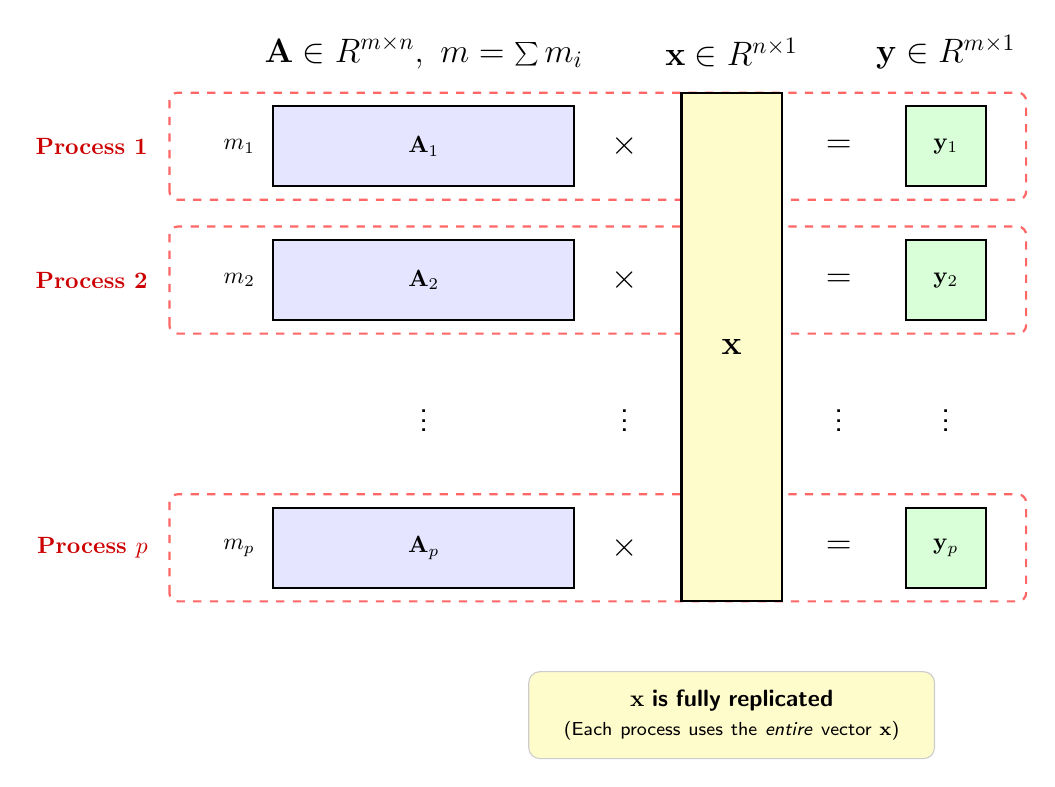
\begin{tikzpicture}[scale=0.85, every node/.style={transform shape}, font=\sffamily]

    % Define reusable styles for the matrices
    \tikzset{
        matA/.style={draw=black, fill=blue!10, thick, minimum width=4.5cm, minimum height=1.2cm, align=center},
        matX/.style={draw=black, fill=yellow!20, thick, minimum width=1.5cm, minimum height=7.6cm, align=center},
        matY/.style={draw=black, fill=green!15, thick, minimum width=1.2cm, minimum height=1.2cm, align=center},
        procbox/.style={draw=red!60, dashed, thick, rounded corners=3pt}
    }

    % =========================================================
    % 1. BACKGROUND PROCESS BOXES
    % =========================================================
    \draw[procbox] (-3.8, 3.2) rectangle (9.0, 4.8);
    \draw[procbox] (-3.8, 1.2) rectangle (9.0, 2.8);
    \draw[procbox] (-3.8, -2.8) rectangle (9.0, -1.2);

    % Process Labels 
    \node[left, text=red!80!black, font=\bfseries] at (-4.0, 4) {Process 1};
    \node[left, text=red!80!black, font=\bfseries] at (-4.0, 2) {Process 2};
    \node[left, text=red!80!black, font=\bfseries] at (-4.0, -2) {Process $p$};

    % =========================================================
    % 2. MATHEMATICAL HEADERS
    % =========================================================
    \node at (0, 5.4) {\Large $\mathbf{A} \in \mathbb{R}^{m \times n}, \ m = \sum m_i$};
    \node at (4.6, 5.4) {\Large $\mathbf{x} \in \mathbb{R}^{n \times 1}$};
    \node at (7.8, 5.4) {\Large $\mathbf{y} \in \mathbb{R}^{m \times 1}$};

    % =========================================================
    % 3. MATRIX A (Distributed Block-Rows)
    % =========================================================
    \node[matA] (A1) at (0, 4) {$\mathbf{A}_1$};
    \node[matA] (A2) at (0, 2) {$\mathbf{A}_2$};
    \node at (0, 0) {\Large $\vdots$};
    \node[matA] (Ap) at (0, -2) {$\mathbf{A}_p$};

    % Local row dimensions (m_i)
    \node[left] at (-2.4, 4) {$m_1$};
    \node[left] at (-2.4, 2) {$m_2$};
    \node[left] at (-2.4, -2) {$m_p$};

    % =========================================================
    % 4. MATH OPERATORS (Per Process)
    % =========================================================
    % Process 1
    \node at (3.0, 4) {\Large $\times$};
    \node at (6.2, 4) {\Large $=$};
    
    % Process 2
    \node at (3.0, 2) {\Large $\times$};
    \node at (6.2, 2) {\Large $=$};
    
    % Ellipses for operators to maintain grid alignment
    \node at (3.0, 0) {\Large $\vdots$};
    \node at (6.2, 0) {\Large $\vdots$};
    
    % Process p
    \node at (3.0, -2) {\Large $\times$};
    \node at (6.2, -2) {\Large $=$};

    % =========================================================
    % 5. VECTOR Y (Distributed Local Results)
    % =========================================================
    \node[matY] (Y1) at (7.8, 4) {$\mathbf{y}_1$};
    \node[matY] (Y2) at (7.8, 2) {$\mathbf{y}_2$};
    \node at (7.8, 0) {\Large $\vdots$};
    \node[matY] (Yp) at (7.8, -2) {$\mathbf{y}_p$};

    % =========================================================
    % 6. VECTOR X (Central / Replicated)
    % Drawn last so it cleanly overlays the dashed boundaries
    % =========================================================
    \node[matX] (X) at (4.6, 1) {\Large $\mathbf{x}$};
    
    % Explanation box safely positioned below the entire diagram
    \node[fill=yellow!20, rounded corners, inner sep=8pt, align=center, text width=5.5cm, draw=black!20] 
        at (4.6, -4.5) {\textbf{$\mathbf{x}$ is fully replicated}\\ \footnotesize (Each process uses the \emph{entire} vector $\mathbf{x}$)};

\end{tikzpicture}
\caption{Distributed block-row matrix-vector product. Matrix $\mathbf{A}$ 
  and result vector $\mathbf{y}$ are partitioned across $p$ processes.
The entire vector $\mathbf{x}$ is required at each node, represented 
by the single unbroken block spanning all processes. This architecture 
minimizes decreases the computations and memory costs per node by $p$.}
\label{fig:distributed_spmv_refined}
\end{figure}

\section{Convergence speed}
\label{sec:ch5-convergence}
The convergence discussion is driven by the spectrum of $\mathbf{A}$.

\begin{theorem}
\label{thm:ch5-spectral-properties}
The following spectral facts hold for linear CG.
\begin{enumerate}
  \item If $\mathbf{A}$ has only $r$ distinct eigenvalues, then CG converges in
  at most $r$ iterations.
  \item If the eigenvalues form a few tight clusters, then in practice CG often
  converges in about the number of clusters rather than in the full dimension.
  \item If $\mu=\lambda_{\min}(\mathbf{A})$ and $L=\lambda_{\max}(\mathbf{A})$,
  then the quadratic \eqref{eq:ch5-quadratic} is $\mu$-strongly convex and
  $L$-smooth, and the classical CG estimate is
  \[
    f(\mathbf{x}_k)-f(\mathbf{x}^\star)
    \le 4
    \left(\frac{\sqrt{L/\mu}-1}{\sqrt{L/\mu}+1}\right)^{2k}
    \bigl(f(\mathbf{x}_0)-f(\mathbf{x}^\star)\bigr).
  \]
 \end{enumerate}
\end{theorem}

The third item is the clean comparison with Chapter~2. Gradient descent has a
linear rate with factor $1-\mu/L$; see \cref{thm:linear-rate}. CG replaces the
dependence on $\kappa=L/\mu$ by a much milder dependence on $\sqrt{\kappa}$.  
Also,
the estimate is quite pessimistic and not very accurate, so in practice algorithm
may be faster.

\begin{example}[Conditioning experiment]
Take
\[
  f(\mathbf{x})=\frac12 \mathbf{x}^{\top}\mathbf{A}\mathbf{x}
  -\mathbf{b}^{\top}\mathbf{x},
  \qquad
  \mathbf{A}=\operatorname{Diag}(a_1,\ldots,a_n),
  \qquad
  \mathbf{b}\sim \mathcal{N}(0,\mathbf{I}_n),
\]
with
\[
  a_i=
  \begin{cases}
    1, & i=1,\\
    \xi_i,\ \xi_i\sim \operatorname{Unif}(1,\kappa), & 2\le i\le n-1,\\
    \kappa, & i=n.
  \end{cases}
\]
Compare the iteration counts of gradient descent and CG as the condition number
$\kappa$ increases.
\end{example}

\begin{figure}[ht]
  \centering
  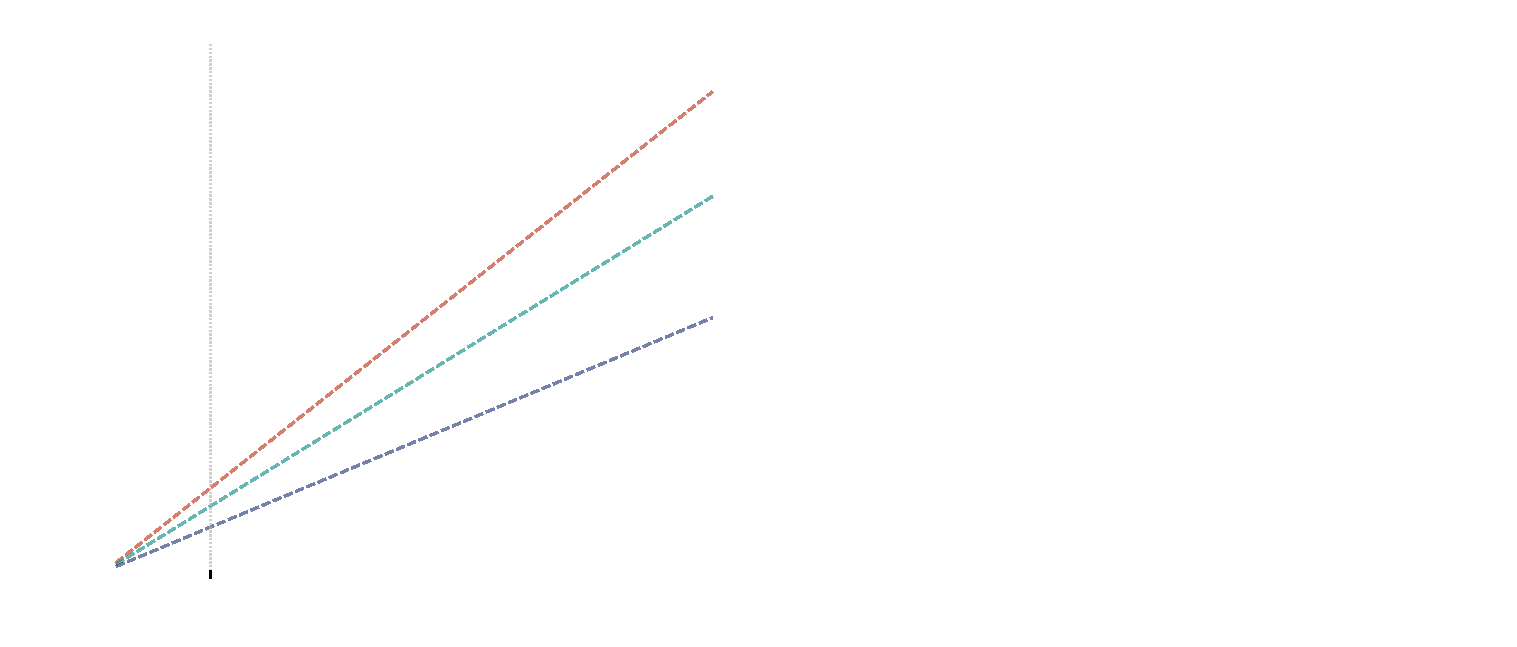
\includegraphics[width=\linewidth]{linear-cg-behaviour.pdf}
  \caption{A conditioning experiment for gradient descent and conjugate
  gradient. Left: for
  gradient descent the iteration count grows roughly linearly with the
  condition number. Right: for CG the dependence is much weaker, the count
  stays bounded by $n$ in exact arithmetic, and increasing the dimension is far
  less damaging than for gradient descent.}
  \label{fig:ch5-linear-cg-behaviour}
\end{figure}

\section{Preconditioning}
\label{sec:ch5-preconditioning}
The next practical question is obvious: what if the matrix is SPD but still
badly conditioned? The answer is to change variables so that CG sees a more
favorable matrix.

Let $\mathbf{S}$ be invertible and define
\[
  \tilde{\mathbf{x}}:=\mathbf{S}\mathbf{x}.
\]
Then
\[
  \mathbf{A}\mathbf{x}=\mathbf{b}
  \quad \Longleftrightarrow \quad
  \underbrace{\mathbf{S}^{-\top}\mathbf{A}\mathbf{S}^{-1}}_{=:\tilde{\mathbf{A}}}
  \tilde{\mathbf{x}}
  =
  \underbrace{\mathbf{S}^{-\top}\mathbf{b}}_{=:\tilde{\mathbf{b}}}.
\]
If $\mathbf{S}$ is chosen so that $\tilde{\mathbf{A}}$ is much better
conditioned than $\mathbf{A}$, then CG on the transformed problem should
converge much faster.

It is convenient to encode this change of variables through the
\emph{preconditioner}
\[
  \mathbf{M}:=\mathbf{S}^{\top}\mathbf{S}.
\]
The ideal case would be $\mathbf{M}=\mathbf{A}$, because then
\[
  \tilde{\mathbf{A}}
  =\mathbf{S}^{-\top}\mathbf{A}\mathbf{S}^{-1}
  =\mathbf{I}.
\]
Of course, the ideal preconditioner is usually as hard to build as solving the
original problem, so in practice one looks for a matrix that is only an
approximation to $\mathbf{A}$ but is cheap to invert or apply.

Running linear CG in the transformed variables and mapping the formulas back
gives the preconditioned recurrence
\[
  \mathbf{d}_0=-\mathbf{M}^{-1}\mathbf{g}_0,
  \qquad
  \mathbf{d}_{k+1}=-\mathbf{M}^{-1}\mathbf{g}_{k+1}+\beta_k \mathbf{d}_k.
\]
If we define
\[
  \mathbf{z}_k:=\mathbf{M}^{-1}\mathbf{g}_k,
\]
then the coefficients become
\begin{equation}
  \label{eq:ch5-pcg-coeffs}
  \alpha_k=\frac{\mathbf{g}_k^{\top}\mathbf{z}_k}
  {\mathbf{d}_k^{\top}\mathbf{A}\mathbf{d}_k},
  \qquad
  \beta_k=\frac{\mathbf{g}_{k+1}^{\top}\mathbf{z}_{k+1}}
  {\mathbf{g}_k^{\top}\mathbf{z}_k}.
\end{equation}

\begin{algorithm}[ht]
  \caption{\textsc{Preconditioned Conjugate Gradient}}
  \label{alg:ch5-pcg}
  \begin{algorithmic}
    \REQUIRE SPD matrix $\mathbf{A}$, right-hand side $\mathbf{b}$, SPD preconditioner $\mathbf{M}$, initial guess $\mathbf{x}_0$, tolerance $\varepsilon>0$
    \STATE $\mathbf{g}_0\gets \mathbf{A}\mathbf{x}_0-\mathbf{b}$, \ $\mathbf{z}_0\gets \mathbf{M}^{-1}\mathbf{g}_0$, \ $\mathbf{d}_0\gets -\mathbf{z}_0$, \ $k\gets 0$
    \WHILE{$\|\mathbf{g}_k\|>\varepsilon$}
      \STATE $\alpha_k\gets \dfrac{\mathbf{g}_k^{\top}\mathbf{z}_k}{\mathbf{d}_k^{\top}\mathbf{A}\mathbf{d}_k}$
      \STATE $\mathbf{x}_{k+1}\gets \mathbf{x}_k+\alpha_k \mathbf{d}_k$
      \STATE $\mathbf{g}_{k+1}\gets \mathbf{g}_k+\alpha_k \mathbf{A}\mathbf{d}_k$
      \STATE $\mathbf{z}_{k+1}\gets \mathbf{M}^{-1}\mathbf{g}_{k+1}$
      \STATE $\beta_k\gets \dfrac{\mathbf{g}_{k+1}^{\top}\mathbf{z}_{k+1}}{\mathbf{g}_k^{\top}\mathbf{z}_k}$
      \STATE $\mathbf{d}_{k+1}\gets -\mathbf{z}_{k+1}+\beta_k \mathbf{d}_k$
      \STATE $k\gets k+1$
    \ENDWHILE
    \RETURN $\mathbf{x}_k$
  \end{algorithmic}
\end{algorithm}

The extra procedure in PCG is the application of $\mathbf{M}^{-1}$ to a
vector. So preconditioning is only worthwhile when
$\mathbf{M}^{-1}\mathbf{v}$ is cheap for the chosen preconditioner.

\begin{example}[Diagonal preconditioning]
Consider
\[
  \mathbf{A}\mathbf{x}=\mathbf{b},
  \qquad
  n=500,
  \qquad
  \mathbf{b}=(1,\ldots,1)^{\top},
\]
with
\[
  a_{ij}=
  \begin{cases}
    1+i^{1.2}, & i=j,\\
    1, & |i-j|=1 \text{ or } |i-j|=100,\\
    0, & \text{otherwise},
  \end{cases}
  \qquad
  \mathbf{M}=\operatorname{Diag}(\mathbf{A}).
\]
This is the simplest diagonal preconditioner.
\end{example}

\begin{figure}[ht]
  \centering
  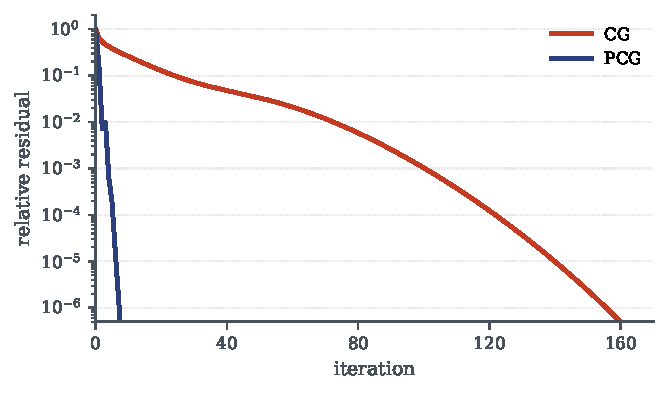
\includegraphics[width=0.74\linewidth]{pcg-example.pdf}
  \caption{A preconditioning example. Even the basic diagonal
  preconditioner $\mathbf{M}=\operatorname{Diag}(\mathbf{A})$ reduces the
  residual much faster than plain CG on the same structured SPD system.}
  \label{fig:ch5-pcg-example}
\end{figure}

This section closes with the right warning: a good preconditioner can
change the behavior of CG completely, but finding such a preconditioner is its
own modeling problem. Typical first options are diagonal scaling and, for
sparse matrices, incomplete Cholesky factorizations that try to preserve the
sparsity pattern.

\section{Nonlinear conjugate gradient}
\label{sec:ch5-nonlinear-cg}
Up to now the quadratic structure has been used everywhere. We now ask what
survives for a general smooth objective $f\in C^1(\mathbb{R}^n)$. The answer
is that the short recurrence survives, but
finite termination disappears and line search becomes an essential part of the
method.

\subsection{Fletcher--Reeves}
Let $\mathbf{g}_k:=\nabla f(\mathbf{x}_k)$. The Fletcher--Reeves version of
nonlinear CG keeps the same update pattern as linear CG:
\[
  \mathbf{d}_0=-\mathbf{g}_0,
  \qquad
  \mathbf{d}_{k+1}=-\mathbf{g}_{k+1}+\beta_k \mathbf{d}_k,
  \qquad
  \beta_k^{\mathrm{FR}}
  =\frac{\mathbf{g}_{k+1}^{\top}\mathbf{g}_{k+1}}
  {\mathbf{g}_k^{\top}\mathbf{g}_k}.
\]
The difference is that the step size is no longer given by
\eqref{eq:ch5-alpha-cg}. One now chooses $\alpha_k$ by a line search, for
example using the Armijo--Wolfe conditions from Chapter~2.

\begin{algorithm}[ht]
  \caption{\textsc{Nonlinear Conjugate Gradient} (Fletcher--Reeves)}
  \label{alg:ch5-nonlinear-cg}
  \begin{algorithmic}
    \REQUIRE $f$, $\nabla f$, initial point $\mathbf{x}_0$, tolerance $\varepsilon>0$
    \STATE $\mathbf{g}_0\gets \nabla f(\mathbf{x}_0)$, \ $\mathbf{d}_0\gets -\mathbf{g}_0$, \ $k\gets 0$
    \WHILE{$\|\mathbf{g}_k\|>\varepsilon \|\nabla f(\mathbf{x}_0)\|$}
      \STATE Choose $\alpha_k$ by a line search
      \STATE $\mathbf{x}_{k+1}\gets \mathbf{x}_k+\alpha_k \mathbf{d}_k$
      \STATE $\mathbf{g}_{k+1}\gets \nabla f(\mathbf{x}_{k+1})$
      \STATE $\beta_k\gets \dfrac{\mathbf{g}_{k+1}^{\top}\mathbf{g}_{k+1}}{\mathbf{g}_k^{\top}\mathbf{g}_k}$
      \STATE $\mathbf{d}_{k+1}\gets -\mathbf{g}_{k+1}+\beta_k \mathbf{d}_k$
      \STATE $k\gets k+1$
    \ENDWHILE
    \RETURN $\mathbf{x}_k$
  \end{algorithmic}
\end{algorithm}

For general objectives, Fletcher--Reeves does \emph{not} automatically
guarantee that every $\mathbf{d}_k$ is a descent direction. A standard
safeguard is to require the strong Wolfe conditions with $c_2<1/2$; then the
generated direction is still a descent direction. This is exactly why the
line-search material from \Cref{alg:expand,alg:zoom} matters here and was not
just a preliminary detour.

\subsection{Other \texorpdfstring{$\beta_k$}{beta} formulas}
Different nonlinear-CG schemes differ only in how the coefficient $\beta_k$ is
chosen. Let
\[
  \mathbf{y}_k:=\mathbf{g}_{k+1}-\mathbf{g}_k.
\]
Common formulas are
\[
\begin{array}{ll}
  \beta_k^{\mathrm{PR}}
  =\dfrac{\mathbf{g}_{k+1}^{\top}\mathbf{y}_k}{\mathbf{g}_k^{\top}\mathbf{g}_k},
  &
  \beta_k^{\mathrm{HS}}
  =\dfrac{\mathbf{g}_{k+1}^{\top}\mathbf{y}_k}{\mathbf{d}_k^{\top}\mathbf{y}_k},
  \\[10pt]
  \beta_k^{\mathrm{PR+}}
  =\max\{0,\beta_k^{\mathrm{PR}}\},
  &
  \beta_k^{\mathrm{GN}}
  =\max\{-\beta_k^{\mathrm{FR}},
  \min(\beta_k^{\mathrm{PR}},\beta_k^{\mathrm{FR}})\},
  \\[10pt]
  \beta_k^{\mathrm{DY}}
  =\dfrac{\mathbf{g}_{k+1}^{\top}\mathbf{g}_{k+1}}{\mathbf{d}_k^{\top}\mathbf{y}_k},
  &
  \beta_k^{\mathrm{HZ}}
  =\dfrac{\left\langle \mathbf{g}_{k+1},
  \mathbf{y}_k
  -2\mathbf{d}_k\frac{\|\mathbf{y}_k\|^2}{\mathbf{d}_k^{\top}\mathbf{y}_k}
  \right\rangle}
  {\mathbf{d}_k^{\top}\mathbf{y}_k}.
\end{array}
\]
On a strictly convex quadratic with exact line search, all of these formulas
collapse to the same method. That is why the linear theory remains the right
local model for nonlinear CG near a quadratic-like minimizer.

\subsection{Restarts}
For a general nonlinear objective, CG no longer finishes in $n$ steps, and the
conjugacy information accumulated in the recurrence can become stale. It is
therefore natural to use occasional restarts:
\[
  \mathbf{d}_k:=-\mathbf{g}_k.
\]
A standard restart condition is
\begin{equation}
  \label{eq:ch5-restart}
  |\mathbf{g}_{k+1}^{\top}\mathbf{g}_k|
  > \nu \|\mathbf{g}_{k+1}\|^2,
  \qquad
  \nu\approx 0.1.
\end{equation}
The idea is simple and geometric: on a quadratic model, neighboring gradients
are orthogonal, so a serious loss of orthogonality is a natural signal to throw
away the accumulated direction history and restart from steepest descent.

\begin{example}[Two standard test problems]
Two standard test problems are:
\begin{itemize}
  \item the Rosenbrock function
  \[
    f(\mathbf{x})=(1-x_1)^2+100(x_2-x_1^2)^2;
  \]
  \item an $\ell_2$-regularized logistic-type objective
  \[
    f(\mathbf{x})
    =\sum_{i=1}^m \ln\bigl(1+\exp(\langle a_i,\mathbf{x}\rangle)\bigr)
    +\frac{\lambda}{2}\|\mathbf{x}\|^2
    \to \min_{\mathbf{x}\in\mathbb{R}^n}.
  \]
\end{itemize}
These two examples illustrate the practical message of nonlinear conjugate
gradient. On
Rosenbrock, plain FR can stall while PR or FR with restart behaves much better;
on a large smooth problem, nonlinear CG can be substantially more effective
than plain gradient descent at the same line-search accuracy.
\end{example}

\begin{figure}[ht]
  \centering
  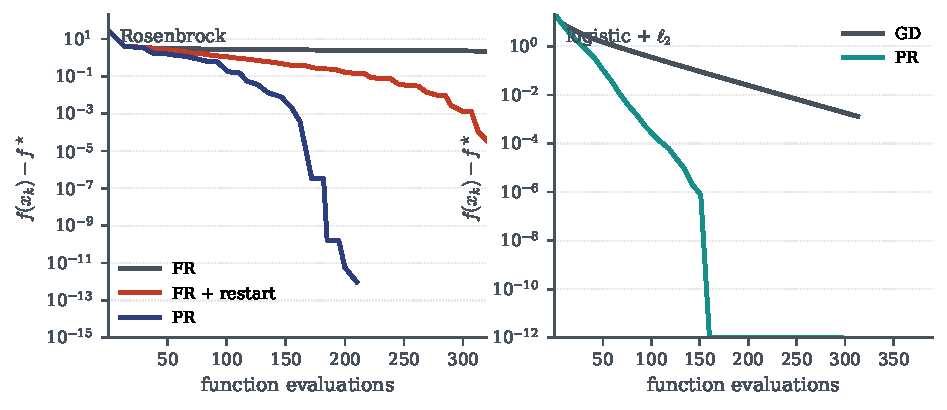
\includegraphics[width=\linewidth]{nonlinear-cg-comparison.pdf}
  \caption{Two nonlinear-CG examples. Left: on Rosenbrock,
  Polak--Ribiere and restarts improve substantially over plain
  Fletcher--Reeves. Right: on a regularized logistic example, nonlinear CG is
  much more effective than gradient descent when measured by function
  evaluations.}
  \label{fig:ch5-nonlinear-cg-comparison}
\end{figure}
